\chapter{METODOLOGI PENELITIAN}	
	\section{Waktu dan Lokasi Penelitian}
	\setlength{\leftskip}{0.7cm}
	Penelitian ini merupakan penelitian berbasis pengembangan (\textit{prototype-based research}) yang dilakukan melalui perancangan, implementasi dan pengujian mandiri secara terkontrol. Studi kasus yang digunakan mengacu pada proses verifikasi dokumen akademik di lingkungan UNIDA Gontor. Adapun pelaksanaan penelitian ini berlangsung dalam rentang waktu bulan Maret hingga Agustus 2026.
		
	% TABLE
	\begin{table}[ht]
	\centering
	\caption{Waktu Penelitian}
	\renewcommand{\arraystretch}{2}

	\begin{tabular}{|c|p{4cm}|c|c|c|c|c|c|}
		\hline
		\textbf{No} &
		\textbf{Jenis Kegiatan} &
		\textbf{Maret} &
		\textbf{April} &
		\textbf{Mei} &
		\textbf{Juni} &
		\textbf{Juli} &
		\textbf{Agustus} \\ \hline		

		1 &
		Penyusunan Proposal Penelitian &
		\cellcolor{blue!70} &
		\cellcolor{blue!70} &
		&
		&
		&
		\\ \hline

		2 &
		Analisis Kebutuhan Sistem dan Protokol Blockchain &
		&
		\cellcolor{blue!70} &
		&
		&
		&
		\\ \hline

		3 &
		Perancangan Smart Contract dan Struktur EIP-712 &
		&
		\cellcolor{blue!70} &
		\cellcolor{blue!70} &
		&
		&
		\\ \hline

		4 &
		Konfigurasi Jaringan Hyperledger Besu dan Mekanisme Zero-gas &
		&
		&
		\cellcolor{blue!70} &
		\cellcolor{blue!70} &
		&
		\\ \hline

		5 &
		Pengembangan Middleware (API) dan Integrasi dengan Protokol EIP-712 &
		&
		&
		&
		\cellcolor{blue!70} &
		\cellcolor{blue!70} &
		\\ \hline

		6 &
		Pengujian Integritas dan Validasi On-Chain &
		&
		&
		&
		&
		\cellcolor{blue!70} &
		\\ \hline

		7 &
		Penyusunan dan Penyelesaian Laporan &
		&
		&
		&
		&
		\cellcolor{blue!70} &
		\cellcolor{blue!70}
		\\ \hline
	\end{tabular}
	\end{table}

	\section{Alat dan Bahan Penelitian}
	
	Kebutuhan sistem yang digunakan dalam pembuatan dan uji coba penelitian ini terbagi menjadi 3 yaitu:
	\begin{secenumerate}
		\item Perangkat Keras:
		\begin{subsecenumerate}
			\item Satu unit Laptop Acer Nitro V16.
			\item Prosesor Intel® Core™ i5-14450HX.
			\item RAM 16 GB.
			\item SSD 512 GB.
		\end{subsecenumerate}
		\item Perangkat Lunak:
		\begin{subsecenumerate}
			\item Foundry Framework: Perangkat pengembangan untuk kompilasi, pengujian, dan deployment Smart Contract.
			\item Visual Studio Code: Sebagai editor kode utama (IDE).
			\item Node.js (LTS Version): Sebagai runtime environment untuk skrip pendukung.
			\item Ether.js v6: Pustaka untuk interaksi antara API middleware dengan Blockchain.
			\item Hyperledger Besu: Software node blockchain privat.
			\item Nest.js: Sebagai framework untuk pembuatan API.
			\item Laravel 13: Sebagai framework untuk pembuatan aplikasi yang berinteraksi dengan user.
			\item Docker dan Docker Compose.
		\end{subsecenumerate}
	\end{secenumerate}
	
	\section{Tahapan Penelitian}
	Penelitian ini menggunakan metode Scrum, yang merupakan salah satu pendekatan dalam \textit{Agile Software Development} yang bersifat iteratif dan incremental. Metode ini dipilih karena mampu mengakomodasi perubahan kebutuhan serta memungkinkan pengembangan sistem dilakukan secara bertahap melalui siklus yang berulang (\textit{Sprint}). Berikut adalah tampilan model Scrum yang tertera pada Gambar \ref{fig:contoh-f}:
	
	\begin{figure}[h!]
		\centering
		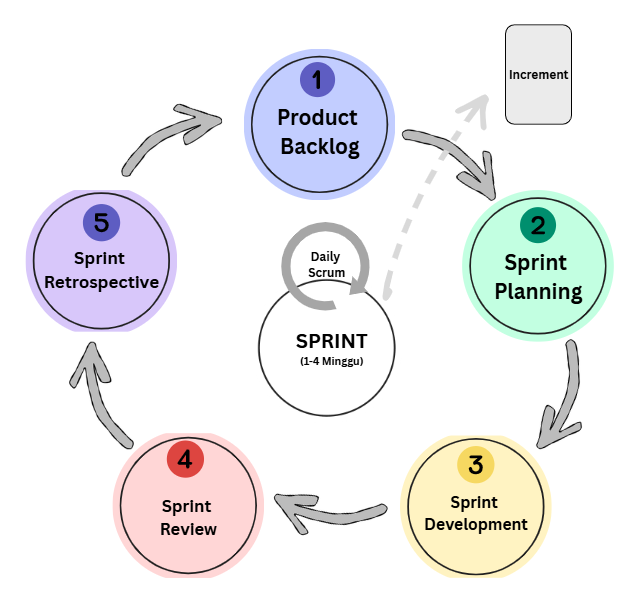
\includegraphics[width=0.8\textwidth]{assets/scrum.png}
		\caption{Metode Scrum}
		\label{fig:contoh-f}
	\end{figure}

		\subsection{Product Backlog}
		\setlength{\leftskip}{1.4cm}
		\textit{Product Backlog} merupakan daftar kebutuhan sistem yang disusun secara terstruktur dan diprioritaskan berdasarkan tingkat kepentingan serta urgensi pengembangan. Daftar ini berisi seluruh fitur dan fungsi yang akan diimplementasikan kedalam sistem, sehingga menjadi acuan dalam pengembangan menggunakan metode Scrum. Penyusunan \textit{Product Backlog} pada penelitian ini dilakukan dengan mempertimbangkan kebutuhan sistem verifikasi berbasis blockchain secara menyeluruh.

		Berdasarkan hasil identifikasi kebutuhan sistem, \textit{Product Backlog} mencakup pembangunan infrastruktur blockchain menggunakan \textit{Hyperledger Besu} dengan mekanisme konsensus QBFT yang mendukung transaksi tanpa biaya (zero gas), konfigurasi node, serta proses deployment smart contract untuk penyimpanan dan verifikasi data dokumen dalam bentuk hash. Selain itu, dirancang struktur metadata dokumen untuk merepresentasikan data akademik secara unik. Tahap selanjutnya meliputi pengembangan smart contract verifikasi, implementasi tanda tangan digital menggunakan EIP-712, serta pembangunan API middleware yang berfungsi sebagai penghubung antara sistem frontend dan jaringan blockchain.

		Selanjutnya, dilakukan integrasi antara middleware dengan blockchain serta pengembangan frontend berbasis Laravel untuk merepresentasikan sistem informasi kampus (SIAKAD Unida). Fitur verifikasi publik juga diimplementasikan agar pengguna eksternal dapat melakukan validasi dokumen tanpa proses autentikasi, namun tetap menjamin keabsahan data. Selain itu, dilakukan pengujian sistem secara menyeluruh, optimasi performa untuk mendukung efisiensi sistem, serta penyusunan dokumentasi sebagai bagian akhir dari pengembangan. Rincian lengkap \textit{Product Backlog} disajikan pada \colorbox{yellow}{tabel 7 2.}

		% TABLE
		\begin{landscape}
			\renewcommand{\arraystretch}{1.3}
			\begin{longtable}{|
			>{\centering\arraybackslash}p{0.8cm}|
			>{\raggedright\arraybackslash}p{4cm}|
			p{8.5cm}|
			>{\centering\arraybackslash}p{2cm}|
			p{5cm}|}

			\caption{Produk Backlog}
			\label{tab:produk_backlog} \\

			\hline
			\textbf{No} &
			\textbf{Product Backlog Item} &
			\textbf{Deskripsi} &
			\textbf{Prioritas} &
			\textbf{Output (Increment)} \\ \hline
			\endfirsthead

			\hline
			\endfoot

			\hline
			\endlastfoot

			% baris
			1 &
			Setup jaringan blockchain (Hyperledger Besu - QBFT) &
			Membangun jaringan blockchain privat menggunakan Hyperledger Besu dengan mekanisme konsensus QBFT untuk mendukung transaksi tanpa biaya (\textit{zero gas}). &
			Tinggi &
			Jaringan blockchain aktif dan dapat digunakan. \\ \hline

			2 &
			Konfigurasi node dan \textit{smart contract deployment} &
			Melakukan konfigurasi node serta proses \textit{deploy smart contract} untuk penyimpanan hash dokumen. &
			Tinggi &
			\textit{Smart contract} berhasil dideploy. \\ \hline

			3 &
			Struktur Data \textit{Typed} &
			Definisi objek JSON terstruktur yang digunakan untuk merepresentasikan data dalam bentuk parameter generik. &
			Tinggi &
			Struktur metadata siap digunakan. \\ \hline

			4 &
			Implementasi \textit{smart contract} verifikasi dokumen &
			Mengembangkan \textit{smart contract} untuk menyimpan dan memverifikasi data dokumen. &
			Tinggi &
			Fungsi verifikasi berjalan di blockchain. \\ \hline

			5 &
			Implementasi EIP-712 &
			Definisi EIP-712 Domain (\textit{Name}, \textit{Version}, \textit{ChainId}, \textit{ContractAddress}). &
			Tinggi &
			Proses \textit{signing} dan \textit{verification} berhasil. \\ \hline

			6 &
			Pengembangan API \textit{middleware} &
			Membangun API sebagai penghubung antara \textit{frontend} dan blockchain (\textit{Relayer}). &
			Tinggi &
			API dapat mengirim dan menerima data. \\ \hline

			7 &
			Integrasi \textit{frontend} (Laravel) &
			Menghubungkan sistem \textit{frontend} dengan API \textit{middleware}. &
			Sedang &
			Antarmuka pengguna dapat berinteraksi dengan sistem. \\ \hline

			9 &
			Implementasi fitur verifikasi publik &
			Mengembangkan fitur verifikasi dokumen tanpa login untuk pengguna eksternal. &
			Tinggi &
			Verifikasi publik dapat digunakan. \\ \hline

			10 &
			Pengujian sistem (\textit{testing}) &
			Melakukan pengujian fungsional dan integrasi sistem. &
			Tinggi &
			Sistem berjalan sesuai kebutuhan. \\ \hline

			12 &
			Dokumentasi sistem &
			Menyusun dokumentasi teknis dan penggunaan sistem. &
			Rendah &
			Dokumentasi sistem tersedia. \\ \hline
				
			\end{longtable}
		\end{landscape}

		\subsection{Sprint Planning}
		Sprint Planning merupakan tahap perencanaan yang dilakukan sebelum Sprint dimulai. Pada tahap ini, dilakukan pemilihan item dari Product Backlog yang akan dikerjakan dalam satu periode Sprint berdasarkan tingkat prioritas yang telah ditentukan. Proses ini bertujuan untuk memastikan bahwa pekerjaan yang dilakukan memiliki fokus yang jelas dan sesuai dengan kebutuhan sistem yang paling mendesak.

		Selain pemilihan backlog, pada tahap ini juga ditentukan tujuan Sprint (Sprint Goal) yang menjadi acuan utama selama proses pengembangan berlangsung. Penentuan tujuan ini penting agar setiap aktivitas yang dilakukan dalam Sprint memiliki arah yang jelas serta dapat memberikan nilai tambah terhadap sistem yang dikembangkan. Dengan adanya Sprint Goal, proses pengembangan menjadi lebih terstruktur dan terukur.

		Selanjutnya, dilakukan pembagian tugas serta perencanaan teknis terkait implementasi fitur yang akan dikembangkan. Dalam konteks penelitian ini, Sprint Planning mencakup perencanaan pengembangan komponen seperti infrastruktur blockchain, smart contract, middleware, serta integrasi sistem. Dengan adanya perencanaan yang matang, diharapkan setiap Sprint dapat menghasilkan Increment yang optimal sesuai dengan target yang telah ditentukan.

		\subsection{Sprint}
		Sprint merupakan inti dari metode Scrum yang berisi seluruh aktivitas pengembangan sistem dalam periode waktu tertentu yang bersifat tetap (time-boxed). Pada tahap ini, seluruh item backlog yang telah dipilih pada Sprint Planning diimplementasikan menjadi bagian sistem yang berfungsi. Aktivitas dalam Sprint mencakup proses pengkodean, integrasi, serta pengujian terhadap fitur yang sedang dikembangkan.

		Selama Sprint berlangsung, dilakukan pertemuan harian yang disebut Daily Scrum untuk memantau perkembangan pekerjaan serta mengidentifikasi hambatan yang dihadapi. Pertemuan ini bertujuan untuk menjaga koordinasi antar proses pengembangan sehingga setiap kendala dapat segera ditangani dan tidak menghambat pencapaian tujuan Sprint.

		Selain itu, pengujian sistem dilakukan secara berkelanjutan selama Sprint untuk memastikan bahwa setiap fitur yang dikembangkan telah berjalan sesuai dengan kebutuhan. Dengan demikian, setiap hasil kerja yang dihasilkan pada akhir Sprint telah memenuhi kriteria yang ditentukan dan siap untuk dievaluasi lebih lanjut pada tahap berikutnya.


		\subsection{Sprint Review}
		Sprint Review merupakan tahap evaluasi yang dilakukan pada akhir Sprint untuk meninjau hasil pengembangan yang telah dicapai. Pada tahap ini, hasil kerja berupa Increment didemonstrasikan untuk memastikan bahwa fitur yang telah dikembangkan sesuai dengan kebutuhan yang telah ditentukan sebelumnya.

		Proses Sprint Review juga berfungsi sebagai sarana untuk memperoleh umpan balik terhadap sistem yang telah dikembangkan. Umpan balik ini sangat penting dalam pengembangan berbasis Scrum karena memungkinkan adanya penyesuaian terhadap kebutuhan sistem yang mungkin berubah selama proses pengembangan berlangsung.

		Hasil dari Sprint Review akan digunakan sebagai dasar untuk memperbarui Product Backlog. Dengan demikian, backlog akan selalu relevan dengan kondisi sistem terkini dan kebutuhan pengguna, sehingga pengembangan pada Sprint berikutnya dapat dilakukan dengan lebih optimal dan terarah.

		\subsection{Sprint Retrospective}
		Sprint Retrospective merupakan tahap evaluasi terhadap proses kerja yang telah dilakukan selama Sprint berlangsung. Fokus utama pada tahap ini adalah mengidentifikasi kelebihan, kekurangan, serta hambatan yang terjadi selama proses pengembangan sistem.

		Pada tahap ini dilakukan analisis terhadap berbagai aspek, seperti efektivitas perencanaan, kendala teknis yang dihadapi, serta koordinasi dalam proses pengembangan. Evaluasi ini bertujuan untuk meningkatkan kualitas proses kerja sehingga Sprint berikutnya dapat berjalan lebih baik dibandingkan sebelumnya.

		Hasil dari Sprint Retrospective digunakan sebagai dasar perbaikan dalam Sprint berikutnya. Dengan adanya evaluasi yang berkelanjutan, metode Scrum memungkinkan peningkatan kualitas sistem secara bertahap, baik dari sisi teknis maupun proses pengembangan.

		\subsection{Increment}
		Sprint Retrospective merupakan tahap evaluasi terhadap proses kerja yang telah dilakukan selama Sprint berlangsung. Fokus utama pada tahap ini adalah mengidentifikasi kelebihan, kekurangan, serta hambatan yang terjadi selama proses pengembangan sistem.

		Pada tahap ini dilakukan analisis terhadap berbagai aspek, seperti efektivitas perencanaan, kendala teknis yang dihadapi, serta koordinasi dalam proses pengembangan. Evaluasi ini bertujuan untuk meningkatkan kualitas proses kerja sehingga Sprint berikutnya dapat berjalan lebih baik dibandingkan sebelumnya.

		yang dihasilkan pada setiap Sprint akan terus dikembangkan dan disempurnakan pada Sprint berikutnya hingga seluruh kebutuhan sistem dalam Product Backlog dapat terpenuhi. Dengan pendekatan ini, sistem yang dibangun menjadi lebih fleksibel, terukur, dan mampu beradaptasi terhadap perubahan kebutuhan selama proses pengembangan berlangsung.

		
	\section{Perancangan Sistem}
		\subsection{Arsitektur Sistem}
		\setlength{\leftskip}{1.4cm}

		Bagian ini menjelaskan rancangan arsitektur sistem yang dibangun untuk mengintegrasikan beberapa komponen utama, seperti SIAKAD Unida, API Middleware, Smart Contract, dan Blockchain. Arsitektur ini dirancang untuk memastikan komunikasi data antra komponen berjalan dengan aman, terdistribusi, dan efisien dalam mendukung verifikasi dokumen akademik. Berikut adalah tampilan arsitektur sistem pada protype, yang tertera pada Gambar 

		\begin{figure}[h!]
			\centering
			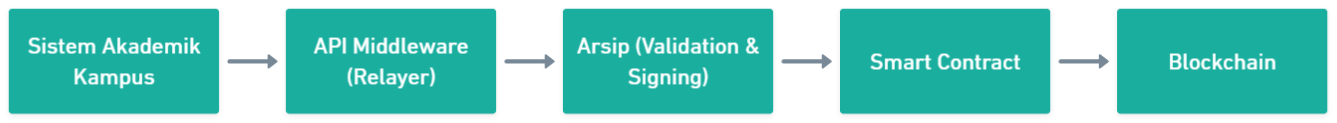
\includegraphics[width=1\textwidth]{assets/arsitektur-utama.png}
			\caption{Arsitektur Sistem}
			\label{fig:contoh-f}
		\end{figure}

		Arsitektur sistem yang dikembangkan terdiri dari beberapa komponen utama yang saling terintegrasi, yang memiliki peran sebagai berikut:

		\begin{subsecenumerate}
			\item Sistem Akademik Kampus: Berperan sebagai sumber utama data dokumen akademik, seperti nomor dokumen, identitas mahasiswa, serta metadata lainnya. Sistem ini berupa SIAKAD Unida atau sistem pengelolaan tentang dokumen akademik. Data yang dihasilkan kemudian dikirimkan ke API Middleware untuk diproses lebih lanjut
			\item API Middleware: Berfungsi sebagai penghubung antara sistem akademik (SIAKAD Unida) dan jaringan blockchain. Komponen ini bertanggung jawab nutuk menerima data dari sistem akademik, melakukan validasi awal, serta mengubah data menjadi format terstruktur yang siap diproses lebih lanjut. Selain itu, middleware juga menyiapkan data menjadi format terstruktur menggunakan protokol EIP-712, sehingga data yang dikirim ke blockchain memiliki integritas dan format yang terstandarisasi. Dalam implementasinya, middleware yang dikembangkan menggunakan Node.js dengan dukungan library Ether.js untuk memfasilitasi interaksi dengan smart contract secara efisien.
			\item Arsip (Validation dan Signing): Pada tahap ini, sistem melakukan validasi dan penandatanganan data dokumen akademik yang akan diarsipkan menggunakan standar protokol EIP-712 dengan kunci privat dari single of authority, yaitu pihak Arsip. Komponen ini mencakup mekanisme validasi integritas dokumen serta proses penandatanganan data secara terstruktur. Selain itu, pendekatan ini menerapkan pemisahan peran antara signer dan relayer untuk memastikan keamanan data dan mengurangi risiko penyalahgunaan kunci pada arsip dokumen.
			\item Smart Contract: Smart contract adalah program yang berjalan diatas jaringan blockchain dan berfungsi sebagai komponen utama untuk verifikasi dokumen. Smart contract bertanggung jawab untuk menerima data yang telah ditandatangani, melakukan dan verifikasi keabsahan suatu dokumen, sehingga meningkatan tranparasi dan kepercayaan terhadap sistem. 
			\item Blockchain: Blockchain sebagai media penyimpanan terdistribusi yang bersifat immutable (tidak dapat dirubah), dalam penelitian ini menggunakan Hyperledger Besu dengan mekanisme konsensus QBFT. Data yang tersimpan di dalam blockchain berupa hash dokumen dan informasi terkait transaksi, sehingga keaslian dokumen dapat diverifikasi kapan saja tanpa resiko manipulasi  
		\end{subsecenumerate}
		
		\subsection{Arsitektur Jaringan Blockchain}
		Arsitektur jaringan blockchain pada sistem ini dirancang menggunakan konsensus Byzantine Fault Tolerance (QBFT) yang berjalan di atas framework Hyperledger Besu. Rancangan ini berokus pada pembagian peran antar node, untuk menjaga kelancaran proses pencatatan data.

		\begin{figure}[h!]
			\centering
			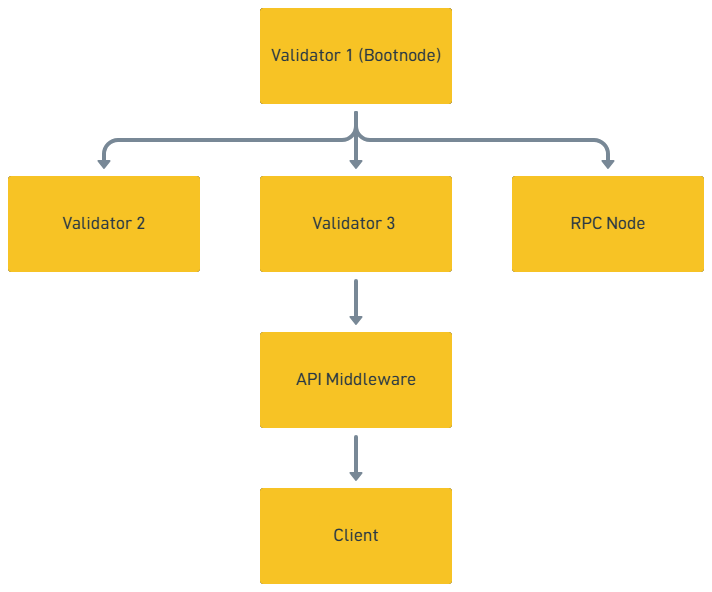
\includegraphics[width=0.8\textwidth]{assets/arsitektur-jaringan.png}
			\caption{Metode Scrum}
			\label{fig:contoh-f}
		\end{figure}

		Berdasarkan visualisasi arsitektur jaringan yang dirancang, berikut adalah penjelasan fungsi dari setiap komponen didalam sistem:

		\begin{subsecenumerate}
			\item Validator 1 (Bootnode): Node utama yang berfungsi sebagai titik awal ketika jaringan di jalankan. Bootnode bertugas mencatat konfigurasi awal jaringan sehingga Validator 2, Validator 3 dan RPC Node dapat saling mengenal.
			\item Validator 2 dan 3: Node penyimpanan yang berfungsi memproses dan mencatat setiap transaksi dokumen baru ke dalam jaringan block.
			\item RPC Node: Node khusus yang bertugas untuk membaca transaksi data pada blockchain, tanpa ikut serta melakukan proses validasi transaksi
		\end{subsecenumerate}

		\subsection{Use Case Sistem}
		Use Case diagram digunakan untuk memodelkan fungsionalitas sistem berdasarkan sudut pandang pengguna. Penjelasan ini menguraikan aktor-aktor yang terlibat serta batasan interaksi mereka dengan sistem. Berikut adalah tampilan Use Case Prototype, yang tertera pada GAMBAR XXX:

		\begin{figure}[h!]
			\centering
			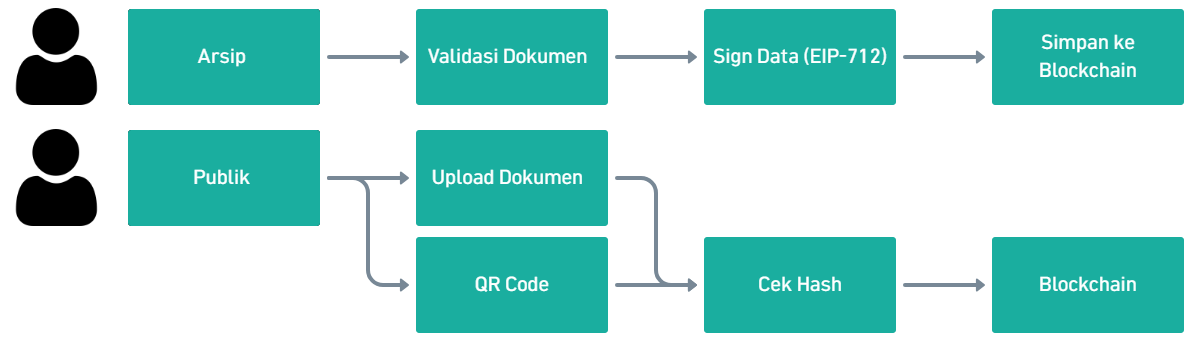
\includegraphics[width=0.8\textwidth]{assets/flow-user.png}
			\caption{Metode Scrum}
			\label{fig:contoh-f}
		\end{figure}

		Berdasarkan diagram alur sistem tersebut, fungsionalitas aplikasi dibagi menjadi dua proses utama yaitu Arsip dan Publik:

		\begin{subsecenumerate}
			\item Alur Arsip: Alur ini menggambarkan proses pengelolaan dokumen oleh pihak biro atau institusi sebagai penerbit dokumen. 
			\begin{subsecenumerate}
				\item Arsip: Proses dimulai dari pihak arsip yang memiliki kewenangan untuk mengelola dan menerbitkan dokumen akademik. Pada tahap ini, dokumen yang akan diverifikasi telah tersedia dalam sistem internal dan siap untuk diproses lebih lanjut. 
				\item Validasi Dokumen: Dokumen yang akan diterbitkan terlebih dahulu melalui proses validasi. Tahap ini bertujuan untuk memastikan bahwa dokumen tersebut sah, lengkap, dan sesuai dengan data yang dimiliki oleh institusi sebelum dilakukan proses digitalisasi ke dalam sistem blockchain.
				\item Sign Data (EIP-712): Setelah dokumen dinyatakan valid, dilakukan proses penandatanganan digital menggunakan standar EIP-712. Mekanisme ini digunakan untuk menjamin keaslian dan integritas data, sehingga dokumen yang telah ditandatangani tidak dapat diubah tanpa terdeteksi.
			\end{subsecenumerate}
			\item Alur Publik: Alur ini menggambarkan proses verifikasi dokumen oleh pengguna eksternal tanpa memerlukan autentikasi khusus.
			\begin{subsecenumerate}
				\item Publik: Proses dimulai dari pengguna eksternal yang ingin melakukan verifikasi terhadap suatu dokumen. Pengguna tidak perlu memiliki akun atau akses khusus untuk menggunakan fitur ini.
				\item Upload Dokumen: Pengguna dapat mengunggah dokumen yang ingin diverifikasi ke dalam sistem. Dokumen ini kemudian akan diproses untuk menghasilkan nilai hash yang akan dibandingkan dengan data yang tersimpan di blockchain.
				\item QR Code: Selain melalui upload dokumen, pengguna juga dapat melakukan verifikasi dengan memindai QR Code yang tertera pada dokumen. QR Code ini berisi informasi atau referensi hash yang telah 	tersimpan sebelumnya.
				\item Cek Hash: Semua metode input (upload, QR Code, atau input manual) akan bermuara pada proses pengecekan hash. Sistem akan membandingkan hash yang diberikan dengan data yang tersimpan di blockchain untuk menentukan keabsahan dokumen.
				\item Blockchain: Tahap akhir adalah proses pencocokan data dengan blockchain. Jika hash ditemukan dan sesuai, maka dokumen dinyatakan valid dan tidak mengalami perubahan. Sebaliknya, jika tidak ditemukan atau tidak sesuai, maka dokumen dianggap tidak valid atau telah dimodifikasi.
			\end{subsecenumerate}

		\end{subsecenumerate}

		\subsection{Flowchart Sistem}
		Flowchart memaparkan urutan logika dan langkah-langkah proses kerja sistem secara terperinci. Bagian ini terbagi menjadi tiga bagian, yaitu: proses penandatanganan, proses verifikasi menggunakan QR Code, dan proses verifikasi manual upload dokumen.

		\begin{subsecenumerate}
			\item Flowchart Penandatanganan Dokumen
				\begin{figure}[H]
					\centering
					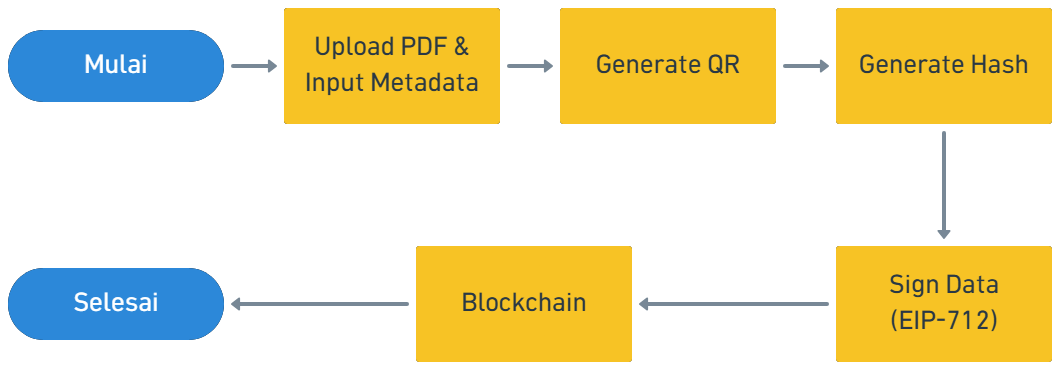
\includegraphics[width=0.9\textwidth]{assets/flowchart-1.png}
					\caption{FLowchart Penandatanganan Digital}
					\label{fig:flowchart-1}
				\end{figure}
				\begin{subsecenumerate}
					\item Upload PDF dan Input Metadata: Pengguna mengunggah berkas mentah PDF sekaligus memasukan informasi pendukung (metadata) dokumen ke dalam sistem secara bersamaan.
					\item Generate QR: Sistem membuat gambar QR Code unik berbasis UUID dan langusung menempelkannya di halaman berkas PDF yang baru diunggah.
					\item Generate HASH: Aplikasi menghitung file hash dari dokumen yang sudah dimuat QR Code didalamnya dan juga informasi pendukung (metadata) menggunakan algoritma SHA-256.
					\item Penandatanganan EIP-712: Proses penandatanganan digital menggunakan standar EIP-712.
					\item Blockchain: Tanda tangan digital dikirim secara permanen ke jaringan blockchain Hyperledger Besu.
				\end{subsecenumerate}
			\item Flowchart Verifikasi Menggunakan QR:
				\begin{figure}[H]
					\centering
					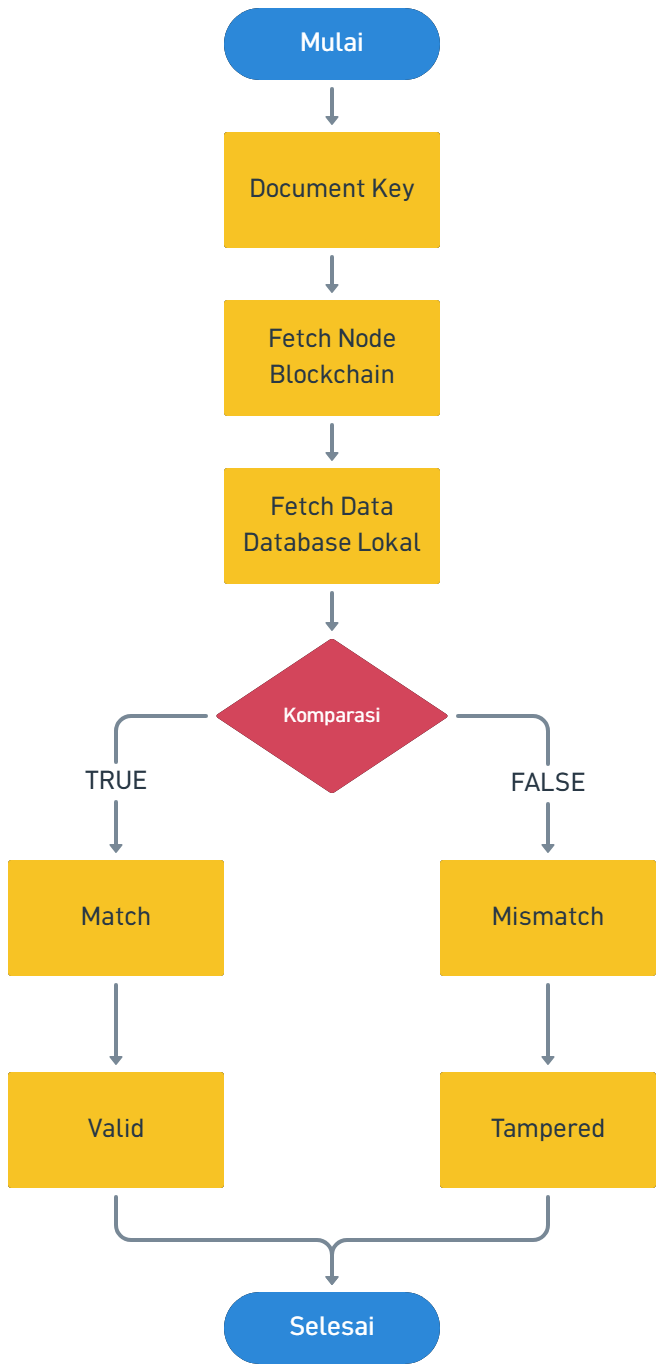
\includegraphics[width=0.5\textwidth]{assets/flowchart-2.png}
					\caption{Flowchart Verifikasi Menggunakan QR}
					\label{fig:flowchart-2}
				\end{figure}
				\begin{subsecenumerate}
					\item Document Key: Sistem mendapatkan document 
					key unik yang dibawa URL dari hasil pemindaian QR tersebut.
					\item Fetch Node Blockchain: Menggunakan document key yang didapatkan, sistem mengambil data status dokumen yang tersimpan secara absolut di dalam jaringan blockchain.
					\item Fetch Data Database Lokal: Secara bersamaan, sistem juga mengambil data dokumen terkait yang tersimpan di database lokal.
					\item Komparasi: Tahap pengujian dimana sistem membadingkan kecocokan data yang diambil dari blockchain dengan data dari database lokal, Valid jika seluruh data tersinkron sepenuhnya, dan bernilai False jika ada data yang belum tersinkron.
				\end{subsecenumerate}
			
			\item Proses Verifikasi Upload Dokumen:
				\begin{figure}[H]
					\centering
					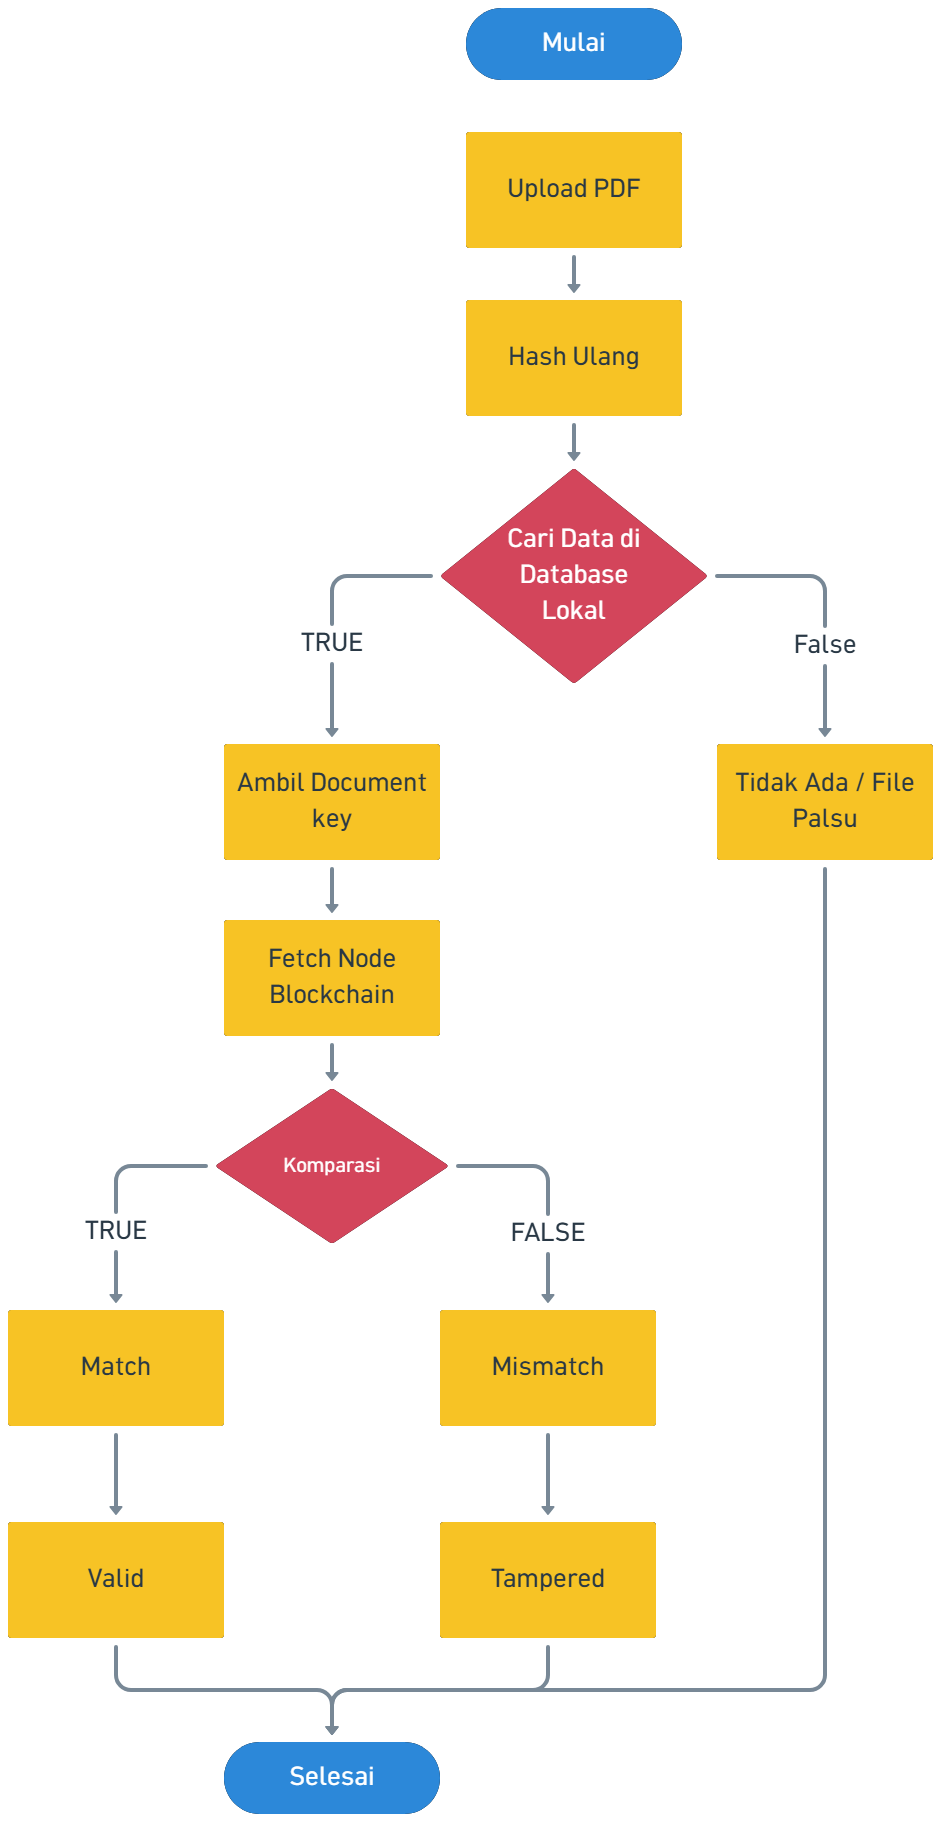
\includegraphics[width=0.6\textwidth]{assets/flowchart-3.png}
					\caption{Proses Verifikasi Upload Dokumen}
					\label{fig:flowchart-3}
				\end{figure}
				\begin{subsecenumerate}
					\item Upload PDF: Pengguna mengunggah berkas pdf yang ingin diperiksa keabsahannya ke dalam sistem.
					\item Hash Ulang: Sistem secara otomatis menghitung kembali nilai dari dokumen tersebut menggunakan algoritma SHA-256 untuk mendapatkan nilai hash terbaru
					\item Cari Data di Database Lokal: Sistem melakukan pencarian record didalam database lokal dengan mencocokannya dengan nilai hash yang baru. False jika nilai hash tidak ditemukan, dan True jika nilai hash cocok dengan data yang ada di database lokal.
					\item Fetch Node Blockchain: Menggunakan documentKey yang diperoleh, sistem melakukan interaksi ke jaringan blockchain untuk menarik data asli yang sudah pernah di masukan ke jaringan.
					\item Komparasi: Sistem membadingkan kecocokan data antara data hash tersebut dengan data hash yang telah diambil dari jaringan blockchain, True jika hasil data dinyatakan sinkron sepenuhnya, dan False jika ada salah satu data tidak sinkron.
				\end{subsecenumerate}

		\end{subsecenumerate}
			
	\section{Pengujian Sistem}
	Proses pengujian dilakukan untuk memvalidasi fungsionalitas sistem, mulai dari penandatanganan data terstruktur hingga transaksi di jaringan privat blockchain. Pengujian ini mencangkup kriptografi EIP-712, evaluasi efisiensi transaksi melalui mekanisme zero-gas pada Hyperledger Besu, verifikasi integritas dokumen pada privat Blockchain, serta pengujian ketahanan manajemen kunci yang memisahkan peran antara pemberi otorisasi dengan pelaksana transaksi. Secara rinci, rencana pengujian prototype pada penelitian ini dijabarkan pada Tabel XXX berikut: 

	% TABLE
	\renewcommand{\arraystretch}{1.3}
	\begin{longtable}{|
	>{\centering\arraybackslash}p{0.8cm}|
	>{\raggedright\arraybackslash}p{2.5cm}|
	p{3.2cm}|
	p{3.2cm}|
	p{3.2cm}|}

	\caption{Rencana Pengujian Sistem}
	\label{tab:rencana_pengujian} \\

	\hline
    \textbf{No} &
    \textbf{Aspek yang Diuji} &
    \textbf{Tujuan Pengujian} &
    \textbf{Metode Pengujian} &
    \textbf{Indikator Keberhasilan} \\ \hline
    \endfirsthead

	\hline
    \endfoot

    \hline
    \endlastfoot

	1 &
    Validitas Tanda Tangan EIP-712 &
    Memastikan \textit{signature} data terstruktur dapat di-\textit{recover} dengan benar. &
    \textit{Black-Box Testing} dengan input data akademik riil. &
    Alamat \textit{signer} hasil \textit{recover} cocok 100\% dengan alamat biro yang terdaftar di kontrak. \\ \hline

    2 &
    Mekanisme Zero-Gas &
    Memastikan transaksi dapat masuk ke blok tanpa memotong saldo \textit{wallet}. &
    Observasi saldo \textit{wallet middleware} sebelum dan sesudah transaksi. &
    Saldo \textit{wallet} tetap statis (tidak berkurang) meskipun status transaksi berhasil/sukses. \\ \hline

    3 &
    Integritas Data \textit{On-Chain} &
    Menilai apakah data akademik tersimpan secara permanen dan valid. &
    Verifikasi \textit{doc\_hash} melalui fungsi \textit{checkDocument} dan \textit{Block Explorer}. &
    Sistem berhasil mengembalikan status \textit{true} untuk hash yang terdaftar dan data tidak dapat diubah. \\ \hline

    4 &
    Manajemen Kunci (\textit{Decoupling}) &
    Memastikan pemisahan peran antara \textit{Signer} dan \textit{Relayer} berfungsi. &
    Simulasi pengiriman transaksi menggunakan \textit{private key} yang berbeda. &
    Transaksi berhasil dieksekusi \textit{on-chain} dengan otorisasi tetap berasal dari kunci biro yang sah. \\ \hline

    5 &
    Konsensus \& \textit{Fault Tolerance} (QBFT) &
    Memastikan jaringan tetap berjalan stabil dengan skema 4 \textit{node} dan 3 validator. &
    Mematikan salah satu \textit{node} validator secara sengaja saat proses transaksi berlangsung. &
    Jaringan tetap mampu menghasilkan blok baru dan memproses transaksi selama minimal 2 validator (2/3) aktif. \\ \hline
		
	\end{longtable}
			